\hypertarget{comparison-of-combat-strategies-through-varied-stochastic-salvo-combat-models}{%
\subsection{Comparison of Combat Strategies Through Varied Stochastic
Salvo Combat
Models}\label{comparison-of-combat-strategies-through-varied-stochastic-salvo-combat-models}}

\hypertarget{scenario}{%
\subsubsection{Scenario}\label{scenario}}

When it comes to warfare, where should navies invest their money? Is it
most important to have more ships? How about more powerful guns, better
targeting systems or stronger armor? There are many considerations that
go in to broad strategic planning, but the scope of this investigation
will be limited to the implications of these differing strategies on
direct military outcomes.

This investigation will consider several theoretical battles between two
navies with differing advantages. Multiple simulations with normally
distributed random differences in coefficient values will be used to
construct a model through which to judge which strategy would come out
on top in a battle between two belligerents of similar means with
different resource allocation strategies.

\hypertarget{background-equations}{%
\subsubsection{Background \& Equations}\label{background-equations}}

In the traditional Salvo combat model, it is assumed that both parties
have accurate targeting systems, allowing for all of its firepower to be
effectively utilized during each combat phase. While this may have been
a fine methodology in decades past when one could assume that any two
belligerents would have an approximately equal chance of striking
accurately, the more recent rise of information driven warfare means
that some sort of measure of targeting capabilities is crucial to the
integrity of the model. This is accomplished in our variant of the salvo
combat model by adding variables to represent the relative accuracy of
each force.

Let's start by defining the terms of the standard (100\% accuracy) salvo
model. For two opposition forces A and B, the following table explains
the meanings of the different variables:

\begin{longtable}[]{@{}llll@{}}
\toprule
Meaning & A & B & Initial Value Bounds\tabularnewline
\midrule
\endhead
Number of Units & A & B & \([2, 6]\)\tabularnewline
Attacking capability per unit & \(\alpha\) & \(\beta\) &
\([1,4]\)\tabularnewline
Defensive capability per unit & y & z & \([1,3]\)\tabularnewline
Staying power per unit & u & v & \([1,2]\)\tabularnewline
\bottomrule
\end{longtable}

Each of the bounds that we have defined for each variable come from an
experiment carried out by Lucas \& McGunnigle and will provide the basis
for our analysis.

The following equations relate the variables in the table to define the
losses suffered by each force after a single engagement.

\[\Delta B = -\frac{(\alpha A - z B)}{v} \text{ where } 0 \leq -\Delta B \leq B\]
\[\Delta A = -\frac{(\beta B - y A)}{u} \text{ where } 0 \leq -\Delta A \leq A\]

To modify these equations to account for accuracy, we can simply add one
more variable to measure the probability of a hit.

\begin{longtable}[]{@{}llll@{}}
\toprule
Meaning & A & B & Initial Value Bounds\tabularnewline
\midrule
\endhead
\(\ldots\) & \(\ldots\) & \(\ldots\) & \ldots{}\tabularnewline
Accuracy & m & n & \((0.5, 1]\)\tabularnewline
\bottomrule
\end{longtable}

Each of these new variables will act as a ratio bound between 0 and 1
that represents the probability of landing a hit by the that army when
attacking.

\[
\begin{cases}
\frac{dB}{dt} = -\frac{(\alpha m A - z B)}{v} & \text{ where } 0 \leq -\frac{dB}{dt} \leq B \\
\frac{dA}{dt} = -\frac{(\beta n B - y A)}{u} & \text{ where } 0 \leq -\frac{dB}{dt} \leq A \\
\end{cases}
\]

Now the attacking power of each force is tempered by its accuracy, and
we have a system of differential equations.

Now that we have the forms of our differential equations determined, we
are ready to determine values and substitute them in. We will be
simulating battles to consider different advantages and their bearing on
outcomes.

Since we do not have definite values for these and would prefer some
variance in our model to account for our uncertainty, we can carry out a
Monte Carlo simulation. Adding in this variance will also help us
account for the inherent uncertainty of simulating a system that is not
in a controlled environment (like a naval engagement).

\hypertarget{brief-intermission---rationale-for-the-simulation}{%
\subsubsection{Brief Intermission - Rationale for the
Simulation}\label{brief-intermission---rationale-for-the-simulation}}

In each section of our simulation, we will consider different advantages
and attempt to quantify their relative bearings on the outcome. This
will be done by running our simulation with different advantages granted
to each side on each iteration.

\hypertarget{simulation}{%
\subsubsection{Simulation}\label{simulation}}

\hypertarget{introduction}{%
\paragraph{Introduction}\label{introduction}}

First, we will provide a baseline of what several battles with no
defined advantages would look like. This will also provide a template
for what our analyses would look like. Our graphs will range from \(-1\)
to \(1\) on the y axis, with positive values indicating advantage for
Force 1 and negative values indicating advantage for Force 2. A line
intersecting \(y=1\) indicates a total victory for Force 1, with the
converse true for Force 2. This graph is for a total factorial
simulation of all integer combinations (or decimals stepped by \(0.1\)
in the case of accuracy) of the bounds of each variable. The
accompanying printout indicates some basic descriptive statistics about
the the simulation.

\begin{figure}
\hypertarget{fig:refname}{%
\centering
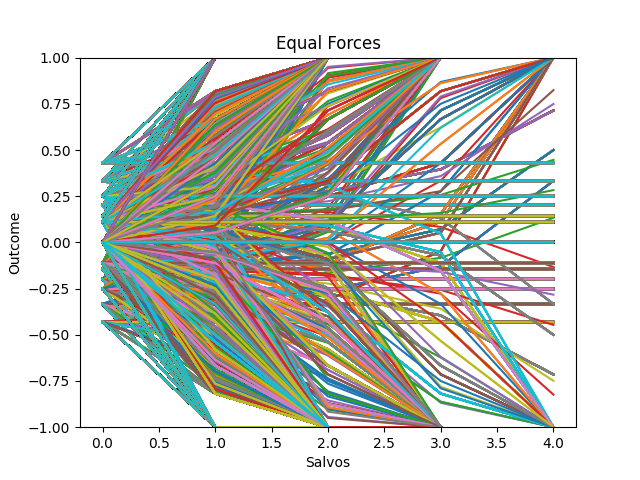
\includegraphics[width=0.6\textwidth,height=\textheight]{figures/EqualForces.png}
\caption{Equal Forces Graph}\label{fig:refname}
}
\end{figure}

\begin{verbatim}
Engagements Simulated: 14400
Force1 Total Victories: 5020
Force2 Total Victories: 5020
Force1 Partial Victories: 1474
Force2 Partial Victories: 1474
Average Score: 0.0
\end{verbatim}

As this simulation was run with no advantage granted to either side, we
see that the number of victories is exactly equal, and our graph is
symmetrical over \(y=0\).

In each of the following simulations we will provide Force1 an advantage
by shifting the bounds of one of its variables. Each simulation will be
capped at a maximum of 5 salvo exchanges.

\hypertarget{example-1-unit-advantage}{%
\paragraph{Example 1: Unit Advantage}\label{example-1-unit-advantage}}

When providing Force1 with a one unit advantage, we see a plot that
visually looks similar to our base plot, but shifted up slightly.

\begin{figure}
\hypertarget{fig:refname}{%
\centering
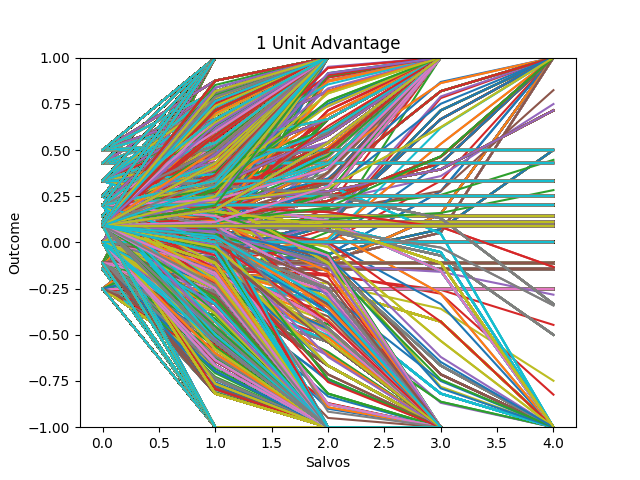
\includegraphics[width=0.6\textwidth,height=\textheight]{figures/1UnitAdv.png}
\caption{1 Unit Advantage}\label{fig:refname}
}
\end{figure}

\begin{verbatim}
Engagements Simulated: 14400
Force1 Total Victories: 7155
Force2 Total Victories: 2959
Force1 Partial Victories: 2264
Force2 Partial Victories: 944
Average Score: 0.5454545454545454
\end{verbatim}

This shows a reasonably large advantage from just having one extra ship.

\hypertarget{example-2-power-advantage}{%
\paragraph{Example 2: Power Advantage}\label{example-2-power-advantage}}

When Force 1 has a one power level advantage, we see an interesting
shift in our outcomes. While the average score difference is less
extreme than with a one unit advantage, a larger proportion of battles
are total victories in Force 1's favor.

\begin{figure}
\hypertarget{fig:refname}{%
\centering
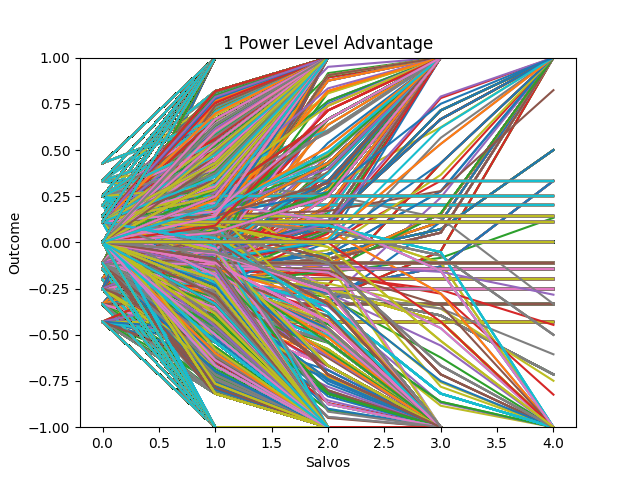
\includegraphics[width=0.6\textwidth,height=\textheight]{figures/1PowerAdv.png}
\caption{1 Power Advantage}\label{fig:refname}
}
\end{figure}

\begin{verbatim}
Engagements Simulated: 14400
Force1 Total Victories: 7825
Force2 Total Victories: 4145
Force1 Partial Victories: 435
Force2 Partial Victories: 1039
Average Score: 0.5
\end{verbatim}

In these cases Force 1, in battles where it has an advantage, has a
heightened ability to destroy Force 2 fully before the time limit
expires, leading to a higher proportion of total victories.

\hypertarget{example-3-one-defense-level-advantage}{%
\paragraph{Example 3: One Defense Level
Advantage}\label{example-3-one-defense-level-advantage}}

While a one defense level advantage yields a higher average score than a
one power level advantage, it achieves this benefit in a much different
way. The number of total victories for Force 1 is much lower than in the
case of a power level advantage but the number of total victories for
Force2 is diminished by an even greater degree.

\begin{figure}
\hypertarget{fig:refname}{%
\centering
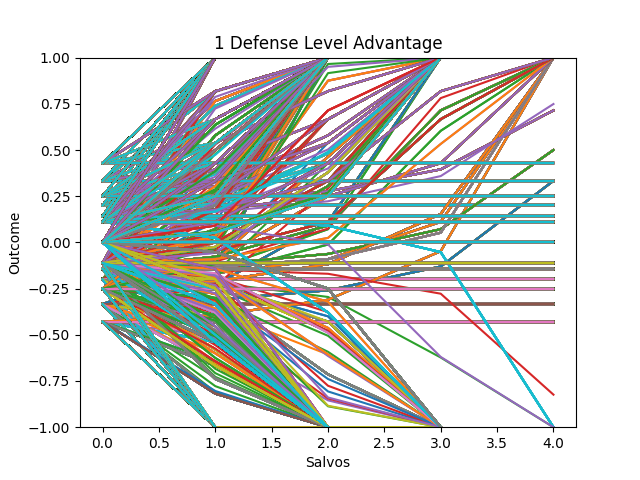
\includegraphics[width=0.6\textwidth,height=\textheight]{figures/1DefenseAdv.png}
\caption{1 Defense Advantage}\label{fig:refname}
}
\end{figure}

\begin{verbatim}
Engagements Simulated: 14400
Force1 Total Victories: 5616
Force2 Total Victories: 2288
Force1 Partial Victories: 1893
Force2 Partial Victories: 2641
Average Score: 0.5128205128205127
\end{verbatim}

Since Force 1 has a much greater capability to intercept missiles
launched by Force 2, it can last much longer in a battle, meaning that
even in cases where it is at a disadvantage it can avoid being
completely wiped out.

\hypertarget{example-4-1-staying-power-level-advantage}{%
\paragraph{Example 4: 1 Staying Power Level
Advantage}\label{example-4-1-staying-power-level-advantage}}

In this case, an advantage in staying power simply provides a more
tempered version of the benefits of greater defense. In a more complex
model (perhaps one where the attacking capabilities of ships are
diminished as they are damaged) staying power may have a different
effect from defense, but in this model that is not the case.

\begin{figure}
\hypertarget{fig:refname}{%
\centering
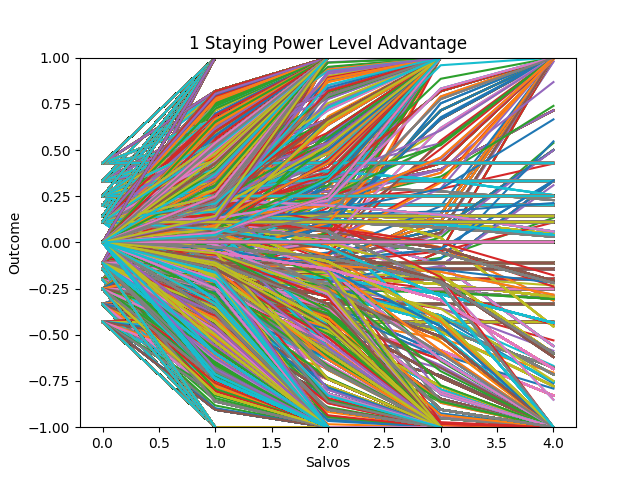
\includegraphics[width=0.6\textwidth,height=\textheight]{figures/1StayingAdv.png}
\caption{1 Staying Power Advantage}\label{fig:refname}
}
\end{figure}

\begin{verbatim}
Engagements Simulated: 14400
Force1 Total Victories: 5337
Force2 Total Victories: 3982
Force1 Partial Victories: 1573
Force2 Partial Victories: 2202
Average Score: 0.45614035087719285
\end{verbatim}

\hypertarget{example-5-1-accuracy-level-0.1-accuracy-advantage}{%
\paragraph{Example 5: 1 Accuracy Level (0.1 Accuracy)
Advantage}\label{example-5-1-accuracy-level-0.1-accuracy-advantage}}

An advantage by one accuracy level has a very interesting effect on the
battle. Even though accuracy is essentially another term for the power
variable, it has a much different effect on the simulation. Even though
the raw difference in the numbers of victories between the two sides is
not very extreme, we see a huge bump in the average score advantage,
indicating that many of the partial victories were severely in favor of
Force 1.

\begin{figure}
\hypertarget{fig:refname}{%
\centering
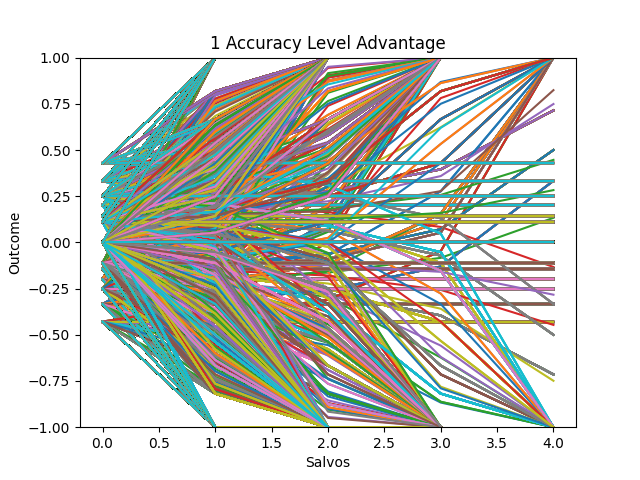
\includegraphics[width=0.6\textwidth,height=\textheight]{figures/1AccuracyAdv.png}
\caption{1 Accuracy Level Advantage}\label{fig:refname}
}
\end{figure}

\begin{verbatim}
Engagements Simulated: 14400
Force1 Total Victories: 5813
Force2 Total Victories: 4789
Force1 Partial Victories: 1154
Force2 Partial Victories: 1347
Average Score: 0.6666666666666659
\end{verbatim}

By examining the graph, we can see that there are many battles that
reach an equilibrium with advantages for Force 1 that don't ever make it
to a total victory, and this is where the bulk of our score difference
lies.

\hypertarget{comparison-of-advantages}{%
\subsubsection{Comparison of
Advantages}\label{comparison-of-advantages}}

Now that we have seen the base impacts that differing advantages have,
we can examine how these advantages interact when pitted against
eachother.

\hypertarget{test-1-turtling-vs-blitzing-defense-vs-attack}{%
\paragraph{Test 1: Turtling vs Blitzing (Defense vs
Attack)}\label{test-1-turtling-vs-blitzing-defense-vs-attack}}

One of the most common (and most infuriating) strategies in Real Time
Strategy video games is ``Turtling,'' or placing a high emphasis on
defensive power to outlast an opponent to the end game. In this
simulation, Force 1 will have a 1 defense level advantage, and Force 2
will have a 1 attack level advantage.

\begin{figure}
\hypertarget{fig:refname}{%
\centering
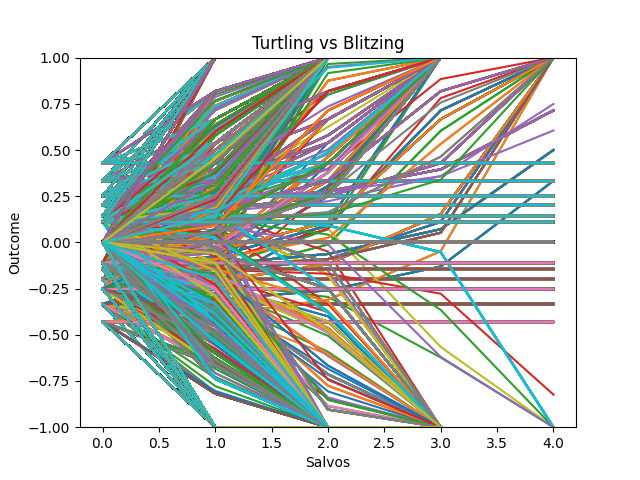
\includegraphics[width=0.6\textwidth,height=\textheight]{figures/turtle.png}
\caption{Turtling vs Blitzing}\label{fig:refname}
}
\end{figure}

\begin{verbatim}
Engagements Simulated: 14400
Force1 Total Victories: 5208
Force2 Total Victories: 4606
Force1 Partial Victories: 1717
Force2 Partial Victories: 1298
Average Score: 0.38095238095238076
\end{verbatim}

In this simulation, we find that better defense does generally win out
over better attack over many battles, but there are some interesting
observations to make. As seen in the graph, many of Force 1 (the
``turtle'')'s victories were won late on, often ending in 3 or 4 salvos
while Force 2 (the ``attacker'')'s victories coming earlier at 1 or 2
exchanges.

\hypertarget{test-2-intel-vs-firepower-accuracy-vs-power}{%
\paragraph{Test 2: Intel vs Firepower (Accuracy vs
Power)}\label{test-2-intel-vs-firepower-accuracy-vs-power}}

This simulation will determine whether it is better to invest in
stronger weapons or better targeting systems, by simulating a battle
between Force 1, who will have an accuracy advantage, and Force 2, who
will have a power advantage.

\begin{figure}
\hypertarget{fig:refname}{%
\centering
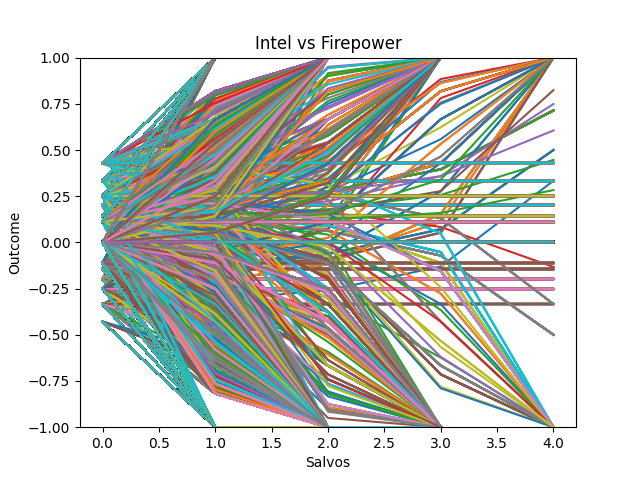
\includegraphics[width=0.6\textwidth,height=\textheight]{figures/IntelVFire.png}
\caption{Intel vs Firepower}\label{fig:refname}
}
\end{figure}

\begin{verbatim}
Engagements Simulated: 14400
Force1 Total Victories: 4770
Force2 Total Victories: 7453
Force1 Partial Victories: 813
Force2 Partial Victories: 383
Average Score: -0.5
\end{verbatim}

While the readout here would suggest a resounding victory for increased
firepower, in truth this simulation is essentially the same as if we
gave both sides unequal power advantages, as power and accuracy are
ultimately multiplied together. The only way to get an accurate handle
on these two statistics would be quantify what the cost to increase each
of these coefficients would be and work from there.

\hypertarget{conclusion}{%
\subsubsection{Conclusion}\label{conclusion}}

Through these various simulations, we found that advantages in different
areas can have starkly different effects on the outcomes of battles.
There are a multitude more tests that could be carried out using this
model and this simulation framework, but this small sampling has already
proven the importance of different strategies.

This model could definitely be improved and expanded upon. Increased
complexity could give a better idea of how these differing advantages
interact (as seen here with the Intel vs Firepower simulation). This
increased complexity could come at the cost of longer simulation times,
as discussed in Lucas \& McGunnigle's paper.

Overall, this has provided some interesting insights in to the
importance of different aspects of naval warfare, and the results of
these simulations seem to have clear and obvious real world analogues,
which is an encouraging indication with regards to the realism of the
model.

\hypertarget{sources}{%
\subsection{Sources}\label{sources}}

\begin{itemize}
\tightlist
\item
  Armstrong, Michael J. ``A Stochastic Salvo Model for Naval Surface
  Combat.'' Operations Research, vol.~53, no. 5, 2005, pp.~830--841.

  \begin{itemize}
  \tightlist
  \item
    Some of the strategies in this paper will be used to consider how to
    deal with accuracy. While the equations here deal with area fire, I
    used them to gain a better idea of how to effectively modify salvo
    with coefficients that won't overpower the base ones.
  \end{itemize}
\item
  Armstrong, Michael J. ``A Stochastic Salvo Model for Naval Surface
  Combat.'' Operations Research, vol.~53, no. 5, 2005, pp.~830--841.

  \begin{itemize}
  \tightlist
  \item
    Some of the strategies in this paper will be used to consider how to
    implement random variation in to our model to allow for multiple
    simulations and a get a better idea of which strategy will prevail.
    Ended up being used mostly as a way to understand what sort of
    variances are appropriate for this type of model rather than
    informing the method used to make the model stochastic.
  \end{itemize}
\item
  Haug, Kevin. (2004). Using Hughes' Salvo Model to Examine Ship
  Characteristics in Surface Warfare. 82.

  \begin{itemize}
  \tightlist
  \item
    This paper provides a great framework for analyzing Salvo warfare
    and also lays out good parameters for bounds on each of the
    coefficients.
  \end{itemize}
\item
  Lucas, T. W., \& McGunnigle, J. E. (2003). When is model complexity
  too much? Illustrating the benefits of simple models with Hughes'
  salvo equations. Naval Research Logistics, 50(3), 197--217.

  \begin{itemize}
  \tightlist
  \item
    This paper provides a great analysis of the traditional Salvo
    Warfare model, which much of my testing is based on.
  \end{itemize}
\end{itemize}
